\documentclass[a4paper]{article}
\usepackage{a4wide}
\usepackage{makeidx}
\usepackage{graphicx}
\usepackage{multicol}
\usepackage{float}
\usepackage{listings}
\usepackage{color}
\usepackage{textcomp}
\usepackage{alltt}
\usepackage{times}
\usepackage{ifpdf}
\ifpdf
\usepackage[pdftex,
            pagebackref=true,
            colorlinks=true,
            linkcolor=blue,
            unicode
           ]{hyperref}
\else
\usepackage[ps2pdf,
            pagebackref=true,
            colorlinks=true,
            linkcolor=blue,
            unicode
           ]{hyperref}
\usepackage{pspicture}
\fi
\usepackage[utf8]{inputenc}
\usepackage{doxygen}
\lstset{language=C++,inputencoding=utf8,basicstyle=\footnotesize,breaklines=true,breakatwhitespace=true,tabsize=8,numbers=left }
\makeindex
\setcounter{tocdepth}{3}
\renewcommand{\footrulewidth}{0.4pt}
\begin{document}
\hypersetup{pageanchor=false}
\begin{titlepage}
\vspace*{7cm}
\begin{center}
{\Large navicom }\\
\vspace*{1cm}
{\large Generated by Doxygen 1.7.1}\\
\vspace*{0.5cm}
{\small Wed May 27 2015 18:05:00}\\
\end{center}
\end{titlepage}
\pagenumbering{roman}
\tableofcontents
\pagenumbering{arabic}
\hypersetup{pageanchor=true}
\section{navicom package documentation}
\label{index}\hypertarget{index}{}The navicom package intends to provide standard methods to visualise high-\/throughput data in NaviCell web service. It also provide several processing method to get some extra meaning out of the data.

\begin{DoxyAuthor}{Author}
Mathurin Dorel 
\end{DoxyAuthor}
\begin{DoxyParagraph}{License: GNU Public License.}

\end{DoxyParagraph}
\hypertarget{main_start}{}\subsection{Getting started}\label{main_start}
The communication with NaviCell web service, and data processing are performed by the \hyperlink{classnavicom_1_1navicom_1_1NaviCom}{NaviCom} class, which can be initialised with a simple NaviCell map URL. 
\begin{DoxyCode}
nc = NaviCom(map\_url=\textcolor{stringliteral}{'https://navicell.curie.fr/navicell/maps/cellcycle/master/in
      dex.php'})
\end{DoxyCode}
 Data and annotations can then be loaded in the \hyperlink{classnavicom_1_1navicom_1_1NaviCom}{NaviCom} object. 
\begin{DoxyCode}
nc.loadData(\textcolor{stringliteral}{"data/Ovarian\_Serous\_Cystadenocarcinoma\_TCGA\_Nature\_2011.txt"})
\end{DoxyCode}
 Two formats are accepted: \begin{DoxyItemize}
\item a matrix format where data are represented as matrix, with explicit rows and columns names. The first row has to start by GENE (for data) or NAME (for annotations); \item a set of matrix format where each matrix is separated by a header line expliciting the type of data and starting with M (data) or ANNOTATIONS (annotations).\end{DoxyItemize}
After being loaded, data and annotations can be easily controlled: 
\begin{DoxyCode}
nc.listData()
nc.listAnnotations()
\end{DoxyCode}
\hypertarget{main_display_config}{}\subsubsection{Display configuration}\label{main_display_config}
The displays in the NaviCell map can be easily configured with the \hyperlink{classnavicom_1_1displayConfig_1_1DisplayConfig}{DisplayConfig} class. It can be provided to the \hyperlink{classnavicom_1_1navicom_1_1NaviCom}{NaviCom} class. 
\begin{DoxyCode}
display\_config = DisplayConfig(5, zero\_color=\textcolor{stringliteral}{"000000"}, na\_color=\textcolor{stringliteral}{"ffffff"}, na\_size
      =0)
nc = NaviCom(map\_url=\textcolor{stringliteral}{'https://navicell.curie.fr/navicell/maps/cellcycle/master/in
      dex.php'}, display\_config)
\end{DoxyCode}
\hypertarget{main_extra_data}{}\subsubsection{Adding extra data}\label{main_extra_data}
Data in the \hyperlink{classnavicom_1_1navicom_1_1NaviCom}{NaviCom} class are represented in the \hyperlink{classnavicom_1_1navidata_1_1NaviData}{NaviData} format, which is a matrix of data that can be indexed by row and column names. \hyperlink{classnavicom_1_1navidata_1_1NaviData}{NaviData} objects can be created independently and integrated to a \hyperlink{classnavicom_1_1navicom_1_1NaviCom}{NaviCom} object: 
\begin{DoxyCode}
extra\_data = NaviData(data\_matrix, row\_names, col\_names)
nc.bindNaviData(extra\_data, \textcolor{stringliteral}{"extra\_data"})
\end{DoxyCode}
\hypertarget{main_visualisation}{}\subsection{Data visualisation}\label{main_visualisation}
The \hyperlink{classnavicom_1_1navicom_1_1NaviCom}{NaviCom} class provides several method to display the data in NaviCell: \begin{DoxyItemize}
\item {\bfseries display} Generic display function to perform any kind of personnalised display \item {\bfseries displayOmics} Display -\/omics data as map staining with extra information or data on using the other display modes \end{DoxyItemize}

\section{Class Index}
\subsection{Class Hierarchy}
This inheritance list is sorted roughly, but not completely, alphabetically:\begin{DoxyCompactList}
\item \contentsline{section}{navicom::displayConfig::DisplayConfig}{\pageref{classnavicom_1_1displayConfig_1_1DisplayConfig}}{}
\item \contentsline{section}{navicom::navicom::NaviCom}{\pageref{classnavicom_1_1navicom_1_1NaviCom}}{}
\item \contentsline{section}{navicom::navidata::NaviData}{\pageref{classnavicom_1_1navidata_1_1NaviData}}{}
\begin{DoxyCompactList}
\item \contentsline{section}{navicom::navidata::NaviAnnotations}{\pageref{classnavicom_1_1navidata_1_1NaviAnnotations}}{}
\end{DoxyCompactList}
\item \contentsline{section}{navicom::navidata::NaviSlice}{\pageref{classnavicom_1_1navidata_1_1NaviSlice}}{}
\end{DoxyCompactList}

\section{Class Index}
\subsection{Class List}
Here are the classes, structs, unions and interfaces with brief descriptions:\begin{DoxyCompactList}
\item\contentsline{section}{\hyperlink{classnavicom_1_1displayConfig_1_1DisplayConfig}{navicom::displayConfig::DisplayConfig} (\hyperlink{classnavicom_1_1displayConfig_1_1DisplayConfig}{DisplayConfig} class to set the color gradients configuration in NaviCell )}{\pageref{classnavicom_1_1displayConfig_1_1DisplayConfig}}{}
\item\contentsline{section}{\hyperlink{classnavicom_1_1navidata_1_1NaviAnnotations}{navicom::navidata::NaviAnnotations} (Enhance \hyperlink{classnavicom_1_1navidata_1_1NaviData}{NaviData} to contain annotations and associate annotations values with samples )}{\pageref{classnavicom_1_1navidata_1_1NaviAnnotations}}{}
\item\contentsline{section}{\hyperlink{classnavicom_1_1navicom_1_1NaviCom}{navicom::navicom::NaviCom} (NaviComm class to handle data and display them in a standardized way on NaviCell maps )}{\pageref{classnavicom_1_1navicom_1_1NaviCom}}{}
\item\contentsline{section}{\hyperlink{classnavicom_1_1navidata_1_1NaviData}{navicom::navidata::NaviData} (Custom class to store the data and be able to access rows and columns by name )}{\pageref{classnavicom_1_1navidata_1_1NaviData}}{}
\item\contentsline{section}{\hyperlink{classnavicom_1_1navidata_1_1NaviSlice}{navicom::navidata::NaviSlice} (A slice from a \hyperlink{classnavicom_1_1navidata_1_1NaviData}{NaviData} array )}{\pageref{classnavicom_1_1navidata_1_1NaviSlice}}{}
\end{DoxyCompactList}

\section{Class Documentation}
\hypertarget{classnavicom_1_1displayConfig_1_1DisplayConfig}{
\subsection{navicom::displayConfig::DisplayConfig Class Reference}
\label{classnavicom_1_1displayConfig_1_1DisplayConfig}\index{navicom::displayConfig::DisplayConfig@{navicom::displayConfig::DisplayConfig}}
}


\hyperlink{classnavicom_1_1displayConfig_1_1DisplayConfig}{DisplayConfig} class to set the color gradients configuration in NaviCell.  


\subsubsection*{Public Member Functions}
\begin{DoxyCompactItemize}
\item 
def \hyperlink{classnavicom_1_1displayConfig_1_1DisplayConfig_a26387ee9e6fe63612bc87a4d5d4a17f2}{\_\-\_\-init\_\-\_\-}
\begin{DoxyCompactList}\small\item\em Initialise a color gradient configuration. \item\end{DoxyCompactList}\item 
\hypertarget{classnavicom_1_1displayConfig_1_1DisplayConfig_ab37d4762509f9ca98fdc74ec06702f36}{
def {\bfseries \_\-\_\-repr\_\-\_\-}}
\label{classnavicom_1_1displayConfig_1_1DisplayConfig_ab37d4762509f9ca98fdc74ec06702f36}

\end{DoxyCompactItemize}
\subsubsection*{Public Attributes}
\begin{DoxyCompactItemize}
\item 
\hypertarget{classnavicom_1_1displayConfig_1_1DisplayConfig_ad8f95c1e3b29ac5622a18b7328b07f50}{
{\bfseries na\_\-color}}
\label{classnavicom_1_1displayConfig_1_1DisplayConfig_ad8f95c1e3b29ac5622a18b7328b07f50}

\item 
\hypertarget{classnavicom_1_1displayConfig_1_1DisplayConfig_aa157506adb33080de983987dd182fa29}{
{\bfseries na\_\-size}}
\label{classnavicom_1_1displayConfig_1_1DisplayConfig_aa157506adb33080de983987dd182fa29}

\item 
\hypertarget{classnavicom_1_1displayConfig_1_1DisplayConfig_aab0e7c765bfc4071416c5e04fd7bbb2f}{
{\bfseries zero\_\-size}}
\label{classnavicom_1_1displayConfig_1_1DisplayConfig_aab0e7c765bfc4071416c5e04fd7bbb2f}

\item 
\hypertarget{classnavicom_1_1displayConfig_1_1DisplayConfig_a86870c1c1b5c920d4cc93554c7528d8a}{
{\bfseries use\_\-absolute\_\-values}}
\label{classnavicom_1_1displayConfig_1_1DisplayConfig_a86870c1c1b5c920d4cc93554c7528d8a}

\item 
\hypertarget{classnavicom_1_1displayConfig_1_1DisplayConfig_a79144928881551fa1f1a18d062d761ea}{
{\bfseries step\_\-count}}
\label{classnavicom_1_1displayConfig_1_1DisplayConfig_a79144928881551fa1f1a18d062d761ea}

\end{DoxyCompactItemize}


\subsubsection{Detailed Description}
\hyperlink{classnavicom_1_1displayConfig_1_1DisplayConfig}{DisplayConfig} class to set the color gradients configuration in NaviCell. 

Definition at line \hyperlink{displayConfig_8py_source_l00051}{51} of file \hyperlink{displayConfig_8py_source}{displayConfig.py}.



\subsubsection{Member Function Documentation}
\hypertarget{classnavicom_1_1displayConfig_1_1DisplayConfig_a26387ee9e6fe63612bc87a4d5d4a17f2}{
\index{navicom::displayConfig::DisplayConfig@{navicom::displayConfig::DisplayConfig}!\_\-\_\-init\_\-\_\-@{\_\-\_\-init\_\-\_\-}}
\index{\_\-\_\-init\_\-\_\-@{\_\-\_\-init\_\-\_\-}!navicom::displayConfig::DisplayConfig@{navicom::displayConfig::DisplayConfig}}
\paragraph[{\_\-\_\-init\_\-\_\-}]{\setlength{\rightskip}{0pt plus 5cm}def navicom::displayConfig::DisplayConfig::\_\-\_\-init\_\-\_\- (
\begin{DoxyParamCaption}
\item[{}]{ self, }
\item[{}]{ step\_\-count = {\ttfamily 3}, }
\item[{}]{ color\_\-gradient = {\ttfamily \mbox{[}\char`\"{}00FF00\char`\"{}}, }
\item[{}]{ FF0000, }
\item[{}]{ zero\_\-color = {\ttfamily \char`\"{}ffffff\char`\"{}}, }
\item[{}]{ na\_\-color = {\ttfamily \char`\"{}ffffff\char`\"{}}, }
\item[{}]{ zero\_\-size = {\ttfamily 0}, }
\item[{}]{ na\_\-size = {\ttfamily 0}, }
\item[{}]{ use\_\-absolute\_\-values = {\ttfamily False}, }
\item[{}]{ excluded = {\ttfamily \char`\"{}10\%\char`\"{}}}
\end{DoxyParamCaption}
)}\hfill}
\label{classnavicom_1_1displayConfig_1_1DisplayConfig_a26387ee9e6fe63612bc87a4d5d4a17f2}


Initialise a color gradient configuration. 


\begin{DoxyParams}{Parameters}
\item[{\em step\_\-count}]number of steps for the color gradients. A step for NAs is automatically attributed. \item[{\em color\_\-gradient}]a list of colors of length 2 or step\_\-count. If length 2 a gradient is built, if the length is step\_\-count the list is used for the colors. \item[{\em zero\_\-color}]an hexadecimal string for the color of the zero, only visible if step\_\-count is odd exclude (str or float): percentage of values to exclude for the color gradient, usefull to avoid a distortion of the colorscale by the extreme values. If str, must match '?'. \end{DoxyParams}


Definition at line \hyperlink{displayConfig_8py_source_l00061}{61} of file \hyperlink{displayConfig_8py_source}{displayConfig.py}.



The documentation for this class was generated from the following file:\begin{DoxyCompactItemize}
\item 
navicom/displayConfig.py\end{DoxyCompactItemize}

\hypertarget{classnavicom_1_1navidata_1_1NaviAnnotations}{
\subsection{navicom::navidata::NaviAnnotations Class Reference}
\label{classnavicom_1_1navidata_1_1NaviAnnotations}\index{navicom::navidata::NaviAnnotations@{navicom::navidata::NaviAnnotations}}
}


Enhance \hyperlink{classnavicom_1_1navidata_1_1NaviData}{NaviData} to contain annotations and associate annotations values with samples.  


Inheritance diagram for navicom::navidata::NaviAnnotations:\begin{figure}[H]
\begin{center}
\leavevmode
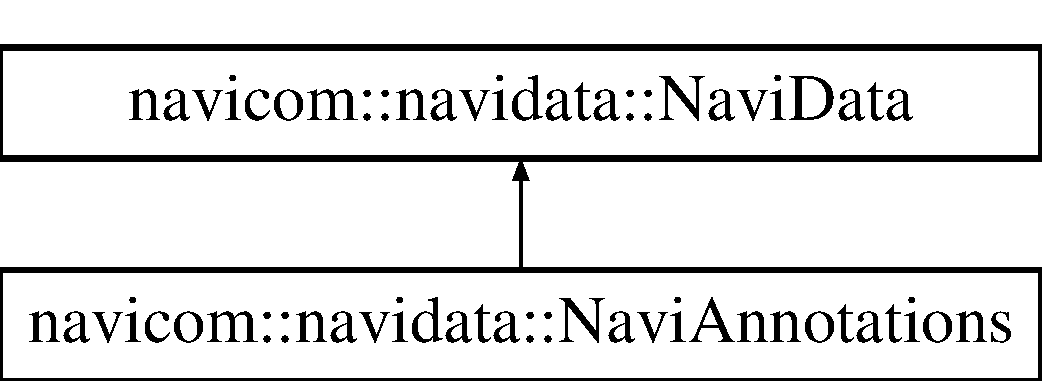
\includegraphics[height=2.000000cm]{classnavicom_1_1navidata_1_1NaviAnnotations}
\end{center}
\end{figure}
\subsubsection*{Public Member Functions}
\begin{DoxyCompactItemize}
\item 
\hypertarget{classnavicom_1_1navidata_1_1NaviAnnotations_a213947a92d3df83acab69c98df419865}{
def {\bfseries \_\-\_\-init\_\-\_\-}}
\label{classnavicom_1_1navidata_1_1NaviAnnotations_a213947a92d3df83acab69c98df419865}

\end{DoxyCompactItemize}
\subsubsection*{Public Attributes}
\begin{DoxyCompactItemize}
\item 
\hypertarget{classnavicom_1_1navidata_1_1NaviAnnotations_a1c26e115cb2eabe4384cd2fa0c7f776f}{
{\bfseries categoriesPerAnnotation}}
\label{classnavicom_1_1navidata_1_1NaviAnnotations_a1c26e115cb2eabe4384cd2fa0c7f776f}

\item 
\hypertarget{classnavicom_1_1navidata_1_1NaviAnnotations_a7cbb4ab623948f19e055f5b4b7c938a9}{
{\bfseries samplesPerCategory}}
\label{classnavicom_1_1navidata_1_1NaviAnnotations_a7cbb4ab623948f19e055f5b4b7c938a9}

\item 
\hypertarget{classnavicom_1_1navidata_1_1NaviAnnotations_ab053ca65505c1a9d72e2afb96ddcae9c}{
{\bfseries old\_\-annots}}
\label{classnavicom_1_1navidata_1_1NaviAnnotations_ab053ca65505c1a9d72e2afb96ddcae9c}

\end{DoxyCompactItemize}


\subsubsection{Detailed Description}
Enhance \hyperlink{classnavicom_1_1navidata_1_1NaviData}{NaviData} to contain annotations and associate annotations values with samples. Also reduce continuous data with to many levels to a limited number of interval levels. 

Definition at line \hyperlink{navidata_8py_source_l00210}{210} of file \hyperlink{navidata_8py_source}{navidata.py}.



The documentation for this class was generated from the following file:\begin{DoxyCompactItemize}
\item 
navicom/navidata.py\end{DoxyCompactItemize}

\hypertarget{classnavicom_1_1navicom_1_1NaviCom}{
\subsection{navicom::navicom::NaviCom Class Reference}
\label{classnavicom_1_1navicom_1_1NaviCom}\index{navicom::navicom::NaviCom@{navicom::navicom::NaviCom}}
}


NaviComm class to handle data and display them in a standardized way on NaviCell maps.  


\subsubsection*{Public Member Functions}
\begin{DoxyCompactItemize}
\item 
def \hyperlink{classnavicom_1_1navicom_1_1NaviCom_ae6133fe7ec63cf5643c1794f4f8e2349}{\_\-\_\-init\_\-\_\-}
\begin{DoxyCompactList}\small\item\em Initialize a Navicell communication object. \item\end{DoxyCompactList}\item 
\hypertarget{classnavicom_1_1navicom_1_1NaviCom_a6eadb16a25ab948c152661c740175383}{
def {\bfseries listData}}
\label{classnavicom_1_1navicom_1_1NaviCom_a6eadb16a25ab948c152661c740175383}

\item 
\hypertarget{classnavicom_1_1navicom_1_1NaviCom_aaf13b634968129b3216c5cb54b70c2ad}{
def {\bfseries listAnnotations}}
\label{classnavicom_1_1navicom_1_1NaviCom_aaf13b634968129b3216c5cb54b70c2ad}

\item 
\hypertarget{classnavicom_1_1navicom_1_1NaviCom_a29ada4f47f518f16ecd59dc569840078}{
def {\bfseries \_\-\_\-repr\_\-\_\-}}
\label{classnavicom_1_1navicom_1_1NaviCom_a29ada4f47f518f16ecd59dc569840078}

\item 
def \hyperlink{classnavicom_1_1navicom_1_1NaviCom_a51ecb41beebc7636bde73be2e1ffc407}{getDataName}
\begin{DoxyCompactList}\small\item\em Return the string identifier corresponding to the data name or tuple. \item\end{DoxyCompactList}\item 
\hypertarget{classnavicom_1_1navicom_1_1NaviCom_ad8ac5b74afb4ceb6ed094604787d4d19}{
def \hyperlink{classnavicom_1_1navicom_1_1NaviCom_ad8ac5b74afb4ceb6ed094604787d4d19}{getDataTuple}}
\label{classnavicom_1_1navicom_1_1NaviCom_ad8ac5b74afb4ceb6ed094604787d4d19}

\begin{DoxyCompactList}\small\item\em Return tuple corresponding to the data name or tuple. \item\end{DoxyCompactList}\item 
def \hyperlink{classnavicom_1_1navicom_1_1NaviCom_ad675e899836271ff4f2fd4bd17ea81d9}{getData}
\begin{DoxyCompactList}\small\item\em Return the NaviData entity corresponding to the data name or tuple. \item\end{DoxyCompactList}\item 
def \hyperlink{classnavicom_1_1navicom_1_1NaviCom_a10e8b8a4c06b4ecf09366ca6b69efff6}{loadData}
\begin{DoxyCompactList}\small\item\em Load data from a .txt or .ncc file containing several datas, or from a .tsv, .ncd or .nca file containing data from one method. \item\end{DoxyCompactList}\item 
def \hyperlink{classnavicom_1_1navicom_1_1NaviCom_ae310adb1d4e8932f0b72b6d8b6ca6301}{bindNaviData}
\begin{DoxyCompactList}\small\item\em Bind a NaviData datatable to the \hyperlink{classnavicom_1_1navicom_1_1NaviCom}{NaviCom} object in order to use it. \item\end{DoxyCompactList}\item 
def \hyperlink{classnavicom_1_1navicom_1_1NaviCom_a5314c49d6b9749693519a4a86cbfde71}{quantifyMutations}
\begin{DoxyCompactList}\small\item\em Transform the qualitative mutation datas into a quantitative one, where 1 means a mutation and 0 no mutation. \item\end{DoxyCompactList}\item 
def \hyperlink{classnavicom_1_1navicom_1_1NaviCom_a6411b52971f15bd11270942cb98eaa1a}{defineModules}
\begin{DoxyCompactList}\small\item\em Defines the modules to use and which module each gene belongs to. \item\end{DoxyCompactList}\item 
\hypertarget{classnavicom_1_1navicom_1_1NaviCom_afd1a299b687bc97e171cff0a738b7b73}{
def \hyperlink{classnavicom_1_1navicom_1_1NaviCom_afd1a299b687bc97e171cff0a738b7b73}{averageModule}}
\label{classnavicom_1_1navicom_1_1NaviCom_afd1a299b687bc97e171cff0a738b7b73}

\begin{DoxyCompactList}\small\item\em Perform module averaging for every modules for one data type. \item\end{DoxyCompactList}\item 
\hypertarget{classnavicom_1_1navicom_1_1NaviCom_a5a59edead26b5d02f17a60df055576f5}{
def \hyperlink{classnavicom_1_1navicom_1_1NaviCom_a5a59edead26b5d02f17a60df055576f5}{exportAnnotations}}
\label{classnavicom_1_1navicom_1_1NaviCom_a5a59edead26b5d02f17a60df055576f5}

\begin{DoxyCompactList}\small\item\em Export samples annotations to NaviCell. \item\end{DoxyCompactList}\item 
def \hyperlink{classnavicom_1_1navicom_1_1NaviCom_ad7d4390d700d4a6d2533647887f8ab94}{display}
\begin{DoxyCompactList}\small\item\em Display data on the NaviCell map. \item\end{DoxyCompactList}\item 
\hypertarget{classnavicom_1_1navicom_1_1NaviCom_a379f15a87ba5c41c3501e9f386102c05}{
def \hyperlink{classnavicom_1_1navicom_1_1NaviCom_a379f15a87ba5c41c3501e9f386102c05}{resetDisplay}}
\label{classnavicom_1_1navicom_1_1NaviCom_a379f15a87ba5c41c3501e9f386102c05}

\begin{DoxyCompactList}\small\item\em Reset the data and samples selections in NaviCell. \item\end{DoxyCompactList}\item 
def \hyperlink{classnavicom_1_1navicom_1_1NaviCom_a018f936de625af8a5dd7e8250ede6483}{displayMethylome}
\begin{DoxyCompactList}\small\item\em Display the methylation data as glyphs or heatmap on the NaviCell map, with mRNA expression of gene CNV as map staining. \item\end{DoxyCompactList}\item 
def \hyperlink{classnavicom_1_1navicom_1_1NaviCom_a01066363389ca01c24f683956f3dc9ad}{displayOmics}
\begin{DoxyCompactList}\small\item\em Display one -\/omics datatable as map staining, with optionnaly some extra information displayed on top (samples as heatmap or barplot, mutations as glyphs, a glyph for the most highly expressed genes, distribution as heatmap). \item\end{DoxyCompactList}\item 
def \hyperlink{classnavicom_1_1navicom_1_1NaviCom_ab539e16bff0a424ebd2753c153ff4e53}{saveAllData}
\begin{DoxyCompactList}\small\item\em Save all data in an .ncc file. \item\end{DoxyCompactList}\item 
\hypertarget{classnavicom_1_1navicom_1_1NaviCom_ac53d9dc53ca0af44586a55fb1bffe8bd}{
def \hyperlink{classnavicom_1_1navicom_1_1NaviCom_ac53d9dc53ca0af44586a55fb1bffe8bd}{saveData}}
\label{classnavicom_1_1navicom_1_1NaviCom_ac53d9dc53ca0af44586a55fb1bffe8bd}

\begin{DoxyCompactList}\small\item\em Save the data in a file that can be exported to NaviCell or imported in \hyperlink{classnavicom_1_1navicom_1_1NaviCom}{NaviCom}. \item\end{DoxyCompactList}\item 
\hypertarget{classnavicom_1_1navicom_1_1NaviCom_aa6a527c98c20f4f75b8529fca178dddc}{
def \hyperlink{classnavicom_1_1navicom_1_1NaviCom_aa6a527c98c20f4f75b8529fca178dddc}{saveAnnotations}}
\label{classnavicom_1_1navicom_1_1NaviCom_aa6a527c98c20f4f75b8529fca178dddc}

\begin{DoxyCompactList}\small\item\em Save the annotations in a file than can be exported to NaviCell or imported in \hyperlink{classnavicom_1_1navicom_1_1NaviCom}{NaviCom}. \item\end{DoxyCompactList}\end{DoxyCompactItemize}
\subsubsection*{Public Attributes}
\begin{DoxyCompactItemize}
\item 
\hypertarget{classnavicom_1_1navicom_1_1NaviCom_a950e5ebf199edea40d55c506b8aaf134}{
\hyperlink{classnavicom_1_1navicom_1_1NaviCom_a950e5ebf199edea40d55c506b8aaf134}{name}}
\label{classnavicom_1_1navicom_1_1NaviCom_a950e5ebf199edea40d55c506b8aaf134}

\begin{DoxyCompactList}\small\item\em Name of the dataset. \item\end{DoxyCompactList}\item 
\hypertarget{classnavicom_1_1navicom_1_1NaviCom_a56141660ddf29a36a8291e938246578c}{
\hyperlink{classnavicom_1_1navicom_1_1NaviCom_a56141660ddf29a36a8291e938246578c}{modules}}
\label{classnavicom_1_1navicom_1_1NaviCom_a56141660ddf29a36a8291e938246578c}

\begin{DoxyCompactList}\small\item\em Composition of the modules. \item\end{DoxyCompactList}\end{DoxyCompactItemize}


\subsubsection{Detailed Description}
NaviComm class to handle data and display them in a standardized way on NaviCell maps. 

Definition at line \hyperlink{navicom_8py_source_l00028}{28} of file \hyperlink{navicom_8py_source}{navicom.py}.



\subsubsection{Member Function Documentation}
\hypertarget{classnavicom_1_1navicom_1_1NaviCom_ae6133fe7ec63cf5643c1794f4f8e2349}{
\index{navicom::navicom::NaviCom@{navicom::navicom::NaviCom}!\_\-\_\-init\_\-\_\-@{\_\-\_\-init\_\-\_\-}}
\index{\_\-\_\-init\_\-\_\-@{\_\-\_\-init\_\-\_\-}!navicom::navicom::NaviCom@{navicom::navicom::NaviCom}}
\paragraph[{\_\-\_\-init\_\-\_\-}]{\setlength{\rightskip}{0pt plus 5cm}def navicom::navicom::NaviCom::\_\-\_\-init\_\-\_\- (
\begin{DoxyParamCaption}
\item[{}]{ self, }
\item[{}]{ map\_\-url = {\ttfamily 'https://navicell.curie.fr/navicell/maps/cellcycle/master/index.php'}, }
\item[{}]{ fname = {\ttfamily \char`\"{}\char`\"{}}, }
\item[{}]{ modules\_\-dict = {\ttfamily \char`\"{}\char`\"{}}, }
\item[{}]{ browser\_\-command = {\ttfamily \char`\"{}firefox~\%s\char`\"{}}, }
\item[{}]{ display\_\-config = {\ttfamily DisplayConfig()}}
\end{DoxyParamCaption}
)}\hfill}
\label{classnavicom_1_1navicom_1_1NaviCom_ae6133fe7ec63cf5643c1794f4f8e2349}


Initialize a Navicell communication object. 


\begin{DoxyParams}{Parameters}
\item[{\em map\_\-url}]URL of the NaviCell map \item[{\em fname}]name of the data file to load \item[{\em modules\_\-dict}]name of the module definition file (.gmt) to load \item[{\em browser\_\-command}]command to open the browser \end{DoxyParams}


Definition at line \hyperlink{navicom_8py_source_l00038}{38} of file \hyperlink{navicom_8py_source}{navicom.py}.

\hypertarget{classnavicom_1_1navicom_1_1NaviCom_ae310adb1d4e8932f0b72b6d8b6ca6301}{
\index{navicom::navicom::NaviCom@{navicom::navicom::NaviCom}!bindNaviData@{bindNaviData}}
\index{bindNaviData@{bindNaviData}!navicom::navicom::NaviCom@{navicom::navicom::NaviCom}}
\paragraph[{bindNaviData}]{\setlength{\rightskip}{0pt plus 5cm}def navicom::navicom::NaviCom::bindNaviData (
\begin{DoxyParamCaption}
\item[{}]{ self, }
\item[{}]{ navidata, }
\item[{}]{ method, }
\item[{}]{ processing}
\end{DoxyParamCaption}
)}\hfill}
\label{classnavicom_1_1navicom_1_1NaviCom_ae310adb1d4e8932f0b72b6d8b6ca6301}


Bind a NaviData datatable to the \hyperlink{classnavicom_1_1navicom_1_1NaviCom}{NaviCom} object in order to use it. 


\begin{DoxyParams}{Parameters}
\item[{\em navidata}]the NaviData datatable to bind \item[{\em method}]the method used to get the data \item[{\em processing}]the visualisation related processing applied to the data \end{DoxyParams}


Definition at line \hyperlink{navicom_8py_source_l00260}{260} of file \hyperlink{navicom_8py_source}{navicom.py}.

\hypertarget{classnavicom_1_1navicom_1_1NaviCom_a6411b52971f15bd11270942cb98eaa1a}{
\index{navicom::navicom::NaviCom@{navicom::navicom::NaviCom}!defineModules@{defineModules}}
\index{defineModules@{defineModules}!navicom::navicom::NaviCom@{navicom::navicom::NaviCom}}
\paragraph[{defineModules}]{\setlength{\rightskip}{0pt plus 5cm}def navicom::navicom::NaviCom::defineModules (
\begin{DoxyParamCaption}
\item[{}]{ self, }
\item[{}]{ modules\_\-dict = {\ttfamily \char`\"{}\char`\"{}}}
\end{DoxyParamCaption}
)}\hfill}
\label{classnavicom_1_1navicom_1_1NaviCom_a6411b52971f15bd11270942cb98eaa1a}


Defines the modules to use and which module each gene belongs to. 


\begin{DoxyParams}{Parameters}
\item[{\em modules\_\-dict}]Either a dict indexed by module name or a file name with the description of each module (.gmt \href{file:}{\tt file:} tab delimited, first column module name, second column description, then list of entities in the module) \end{DoxyParams}


Definition at line \hyperlink{navicom_8py_source_l00308}{308} of file \hyperlink{navicom_8py_source}{navicom.py}.

\hypertarget{classnavicom_1_1navicom_1_1NaviCom_ad7d4390d700d4a6d2533647887f8ab94}{
\index{navicom::navicom::NaviCom@{navicom::navicom::NaviCom}!display@{display}}
\index{display@{display}!navicom::navicom::NaviCom@{navicom::navicom::NaviCom}}
\paragraph[{display}]{\setlength{\rightskip}{0pt plus 5cm}def navicom::navicom::NaviCom::display (
\begin{DoxyParamCaption}
\item[{}]{ self, }
\item[{}]{ perform\_\-list, }
\item[{}]{ default\_\-samples = {\ttfamily \char`\"{}all:~1.0\char`\"{}}, }
\item[{}]{ colors = {\ttfamily \char`\"{}\char`\"{}}, }
\item[{}]{ module = {\ttfamily ''}, }
\item[{}]{ reset = {\ttfamily True}}
\end{DoxyParamCaption}
)}\hfill}
\label{classnavicom_1_1navicom_1_1NaviCom_ad7d4390d700d4a6d2533647887f8ab94}


Display data on the NaviCell map. 

perform\_\-list (list of 2-\/tuples): each tuple must contain the name of the data to display and the mode of display (\char`\"{}glyphN\_\-(color$|$size$|$shape)\char`\"{}, \char`\"{}barplot\char`\"{}, \char`\"{}heatmap\char`\"{} or \char`\"{}map\_\-staining\char`\"{}). Barplots and heatmaps cannot be displayed simultaneously. Several data types can be specified for heatmaps. Specifying \char`\"{}glyph\char`\"{} (without number) will automatically select a new glyph for each data using the same properties (shape, color or size) in glyphs (maximum of 5 glyphs). 
\begin{DoxyParams}{Parameters}
\item[{\em colors}]range of colors to use (NOT IMPLEMENTED YET) default\_\-samples (str or list of str) : Samples to use. Only the first sample is used for glyphs and map staining, all default\_\-samples from the list are used for heatmaps and barplots. Use 'all\_\-samples' to use all default\_\-samples or \mbox{[}'annot1:...:annotn', 'all\_\-groups'\mbox{]} to use all groups corresponding to the combinations of annot1...annotn. \end{DoxyParams}


Definition at line \hyperlink{navicom_8py_source_l00579}{579} of file \hyperlink{navicom_8py_source}{navicom.py}.

\hypertarget{classnavicom_1_1navicom_1_1NaviCom_a018f936de625af8a5dd7e8250ede6483}{
\index{navicom::navicom::NaviCom@{navicom::navicom::NaviCom}!displayMethylome@{displayMethylome}}
\index{displayMethylome@{displayMethylome}!navicom::navicom::NaviCom@{navicom::navicom::NaviCom}}
\paragraph[{displayMethylome}]{\setlength{\rightskip}{0pt plus 5cm}def navicom::navicom::NaviCom::displayMethylome (
\begin{DoxyParamCaption}
\item[{}]{ self, }
\item[{}]{ samples = {\ttfamily \char`\"{}all:~1.0\char`\"{}}, }
\item[{}]{ processing = {\ttfamily \char`\"{}raw\char`\"{}}, }
\item[{}]{ background = {\ttfamily \char`\"{}mRNA\char`\"{}}, }
\item[{}]{ methylation = {\ttfamily \char`\"{}glyph\char`\"{}}}
\end{DoxyParamCaption}
)}\hfill}
\label{classnavicom_1_1navicom_1_1NaviCom_a018f936de625af8a5dd7e8250ede6483}


Display the methylation data as glyphs or heatmap on the NaviCell map, with mRNA expression of gene CNV as map staining. 


\begin{DoxyParams}{Parameters}
\item[{\em background}]should genes, mRNA or no data be used for the map staining \item[{\em processing}]should the processed data be used \end{DoxyParams}


Definition at line \hyperlink{navicom_8py_source_l00886}{886} of file \hyperlink{navicom_8py_source}{navicom.py}.

\hypertarget{classnavicom_1_1navicom_1_1NaviCom_a01066363389ca01c24f683956f3dc9ad}{
\index{navicom::navicom::NaviCom@{navicom::navicom::NaviCom}!displayOmics@{displayOmics}}
\index{displayOmics@{displayOmics}!navicom::navicom::NaviCom@{navicom::navicom::NaviCom}}
\paragraph[{displayOmics}]{\setlength{\rightskip}{0pt plus 5cm}def navicom::navicom::NaviCom::displayOmics (
\begin{DoxyParamCaption}
\item[{}]{ self, }
\item[{}]{ dataName, }
\item[{}]{ group = {\ttfamily \char`\"{}all:~1.0\char`\"{}}, }
\item[{}]{ samplesDisplay = {\ttfamily \char`\"{}\char`\"{}}, }
\item[{}]{ samples = {\ttfamily list()}, }
\item[{}]{ binsNb = {\ttfamily 10}}
\end{DoxyParamCaption}
)}\hfill}
\label{classnavicom_1_1navicom_1_1NaviCom_a01066363389ca01c24f683956f3dc9ad}


Display one -\/omics datatable as map staining, with optionnaly some extra information displayed on top (samples as heatmap or barplot, mutations as glyphs, a glyph for the most highly expressed genes, distribution as heatmap). 

dataName (str or tuple): name or identifier of the data. 
\begin{DoxyParams}{Parameters}
\item[{\em group}]Identifier of the group to display \item[{\em samplesDisplay}]Channel where the individual samples should be displayed (heatmap or barplot) samples (list or str): list of samples to display, or a string specifying how such a list should be built ('quantiles' to get the distribution of values) \item[{\em nbOfSamples}]number of individual samples to display, ignored if samples is a list \end{DoxyParams}


Definition at line \hyperlink{navicom_8py_source_l00927}{927} of file \hyperlink{navicom_8py_source}{navicom.py}.

\hypertarget{classnavicom_1_1navicom_1_1NaviCom_ad675e899836271ff4f2fd4bd17ea81d9}{
\index{navicom::navicom::NaviCom@{navicom::navicom::NaviCom}!getData@{getData}}
\index{getData@{getData}!navicom::navicom::NaviCom@{navicom::navicom::NaviCom}}
\paragraph[{getData}]{\setlength{\rightskip}{0pt plus 5cm}def navicom::navicom::NaviCom::getData (
\begin{DoxyParamCaption}
\item[{}]{ self, }
\item[{}]{ data\_\-name}
\end{DoxyParamCaption}
)}\hfill}
\label{classnavicom_1_1navicom_1_1NaviCom_ad675e899836271ff4f2fd4bd17ea81d9}


Return the NaviData entity corresponding to the data name or tuple. 

data\_\-name (str or tuple): Identifier of the data 

Definition at line \hyperlink{navicom_8py_source_l00140}{140} of file \hyperlink{navicom_8py_source}{navicom.py}.

\hypertarget{classnavicom_1_1navicom_1_1NaviCom_a51ecb41beebc7636bde73be2e1ffc407}{
\index{navicom::navicom::NaviCom@{navicom::navicom::NaviCom}!getDataName@{getDataName}}
\index{getDataName@{getDataName}!navicom::navicom::NaviCom@{navicom::navicom::NaviCom}}
\paragraph[{getDataName}]{\setlength{\rightskip}{0pt plus 5cm}def navicom::navicom::NaviCom::getDataName (
\begin{DoxyParamCaption}
\item[{}]{ self, }
\item[{}]{ data\_\-name}
\end{DoxyParamCaption}
)}\hfill}
\label{classnavicom_1_1navicom_1_1NaviCom_a51ecb41beebc7636bde73be2e1ffc407}


Return the string identifier corresponding to the data name or tuple. 

data\_\-name (str or tuple): Identifier of the data 

Definition at line \hyperlink{navicom_8py_source_l00114}{114} of file \hyperlink{navicom_8py_source}{navicom.py}.

\hypertarget{classnavicom_1_1navicom_1_1NaviCom_a10e8b8a4c06b4ecf09366ca6b69efff6}{
\index{navicom::navicom::NaviCom@{navicom::navicom::NaviCom}!loadData@{loadData}}
\index{loadData@{loadData}!navicom::navicom::NaviCom@{navicom::navicom::NaviCom}}
\paragraph[{loadData}]{\setlength{\rightskip}{0pt plus 5cm}def navicom::navicom::NaviCom::loadData (
\begin{DoxyParamCaption}
\item[{}]{ self, }
\item[{}]{ fname = {\ttfamily \char`\"{}data/Ovarian\_\-Serous\_\-Cystadenocarcinoma\_\-TCGA\_\-Nature\_\-2011.txt\char`\"{}}, }
\item[{}]{ keep\_\-mutations\_\-nan = {\ttfamily False}}
\end{DoxyParamCaption}
)}\hfill}
\label{classnavicom_1_1navicom_1_1NaviCom_a10e8b8a4c06b4ecf09366ca6b69efff6}


Load data from a .txt or .ncc file containing several datas, or from a .tsv, .ncd or .nca file containing data from one method. 


\begin{DoxyParams}{Parameters}
\item[{\em fname}]name of the file from which the data should be loaded \item[{\em keep\_\-mutations\_\-nan}]whether nan in mutations data should be considered as no mutation (False) or missing value (True) \end{DoxyParams}


Definition at line \hyperlink{navicom_8py_source_l00152}{152} of file \hyperlink{navicom_8py_source}{navicom.py}.

\hypertarget{classnavicom_1_1navicom_1_1NaviCom_a5314c49d6b9749693519a4a86cbfde71}{
\index{navicom::navicom::NaviCom@{navicom::navicom::NaviCom}!quantifyMutations@{quantifyMutations}}
\index{quantifyMutations@{quantifyMutations}!navicom::navicom::NaviCom@{navicom::navicom::NaviCom}}
\paragraph[{quantifyMutations}]{\setlength{\rightskip}{0pt plus 5cm}def navicom::navicom::NaviCom::quantifyMutations (
\begin{DoxyParamCaption}
\item[{}]{ self, }
\item[{}]{ method, }
\item[{}]{ keep\_\-nan = {\ttfamily False}}
\end{DoxyParamCaption}
)}\hfill}
\label{classnavicom_1_1navicom_1_1NaviCom_a5314c49d6b9749693519a4a86cbfde71}


Transform the qualitative mutation datas into a quantitative one, where 1 means a mutation and 0 no mutation. 


\begin{DoxyParams}{Parameters}
\item[{\em keep\_\-nan}]Should nan values be converted to O (no mutations) or kept as missing data \end{DoxyParams}


Definition at line \hyperlink{navicom_8py_source_l00285}{285} of file \hyperlink{navicom_8py_source}{navicom.py}.

\hypertarget{classnavicom_1_1navicom_1_1NaviCom_ab539e16bff0a424ebd2753c153ff4e53}{
\index{navicom::navicom::NaviCom@{navicom::navicom::NaviCom}!saveAllData@{saveAllData}}
\index{saveAllData@{saveAllData}!navicom::navicom::NaviCom@{navicom::navicom::NaviCom}}
\paragraph[{saveAllData}]{\setlength{\rightskip}{0pt plus 5cm}def navicom::navicom::NaviCom::saveAllData (
\begin{DoxyParamCaption}
\item[{}]{ self, }
\item[{}]{ folder = {\ttfamily \char`\"{}\char`\"{}}, }
\item[{}]{ indFiles = {\ttfamily False}}
\end{DoxyParamCaption}
)}\hfill}
\label{classnavicom_1_1navicom_1_1NaviCom_ab539e16bff0a424ebd2753c153ff4e53}


Save all data in an .ncc file. 

Does not save the distribution nor color data.


\begin{DoxyParams}{Parameters}
\item[{\em folder}]folder where the data will be save, the name is automatically attributed from the name of the dataset, the method and the processing \item[{\em indFiles}]whether the data should be saved in a single file or in separate files \end{DoxyParams}


Definition at line \hyperlink{navicom_8py_source_l01060}{1060} of file \hyperlink{navicom_8py_source}{navicom.py}.



The documentation for this class was generated from the following file:\begin{DoxyCompactItemize}
\item 
navicom/navicom.py\end{DoxyCompactItemize}

\hypertarget{classnavicom_1_1navidata_1_1NaviData}{
\subsection{navicom::navidata::NaviData Class Reference}
\label{classnavicom_1_1navidata_1_1NaviData}\index{navicom::navidata::NaviData@{navicom::navidata::NaviData}}
}


Custom class to store the data and be able to access rows and columns by name.  


Inheritance diagram for navicom::navidata::NaviData:\begin{figure}[H]
\begin{center}
\leavevmode
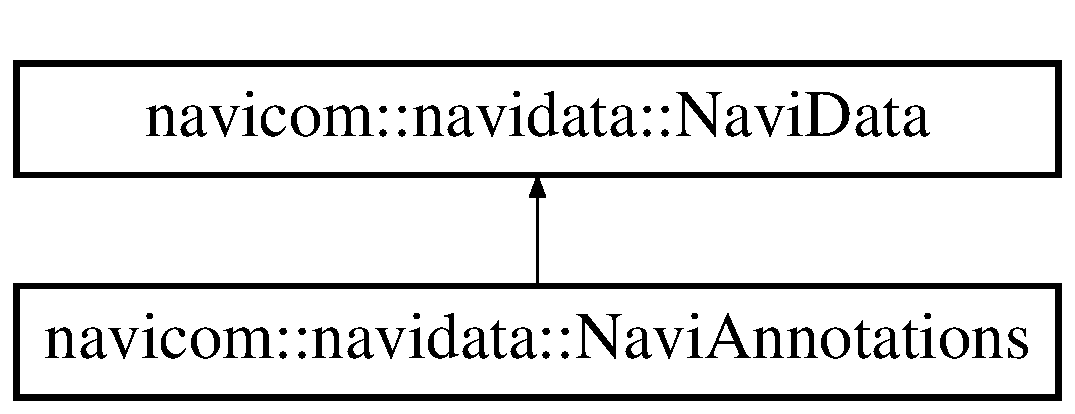
\includegraphics[height=2.000000cm]{classnavicom_1_1navidata_1_1NaviData}
\end{center}
\end{figure}
\subsubsection*{Public Member Functions}
\begin{DoxyCompactItemize}
\item 
\hypertarget{classnavicom_1_1navidata_1_1NaviData_a7daecf05013e46441e7a2d2c935e7a87}{
def {\bfseries \_\-\_\-init\_\-\_\-}}
\label{classnavicom_1_1navidata_1_1NaviData_a7daecf05013e46441e7a2d2c935e7a87}

\item 
\hypertarget{classnavicom_1_1navidata_1_1NaviData_aa01878cdfddf20a588a5ecb48aed373d}{
def {\bfseries \_\-\_\-getitem\_\-\_\-}}
\label{classnavicom_1_1navidata_1_1NaviData_aa01878cdfddf20a588a5ecb48aed373d}

\item 
\hypertarget{classnavicom_1_1navidata_1_1NaviData_a840a803d8e1057ef6702283e8c3033ec}{
def {\bfseries \_\-\_\-iter\_\-\_\-}}
\label{classnavicom_1_1navidata_1_1NaviData_a840a803d8e1057ef6702283e8c3033ec}

\item 
\hypertarget{classnavicom_1_1navidata_1_1NaviData_a45175594977364139b3ad8d0f20db010}{
def {\bfseries \_\-\_\-next\_\-\_\-}}
\label{classnavicom_1_1navidata_1_1NaviData_a45175594977364139b3ad8d0f20db010}

\item 
\hypertarget{classnavicom_1_1navidata_1_1NaviData_a5780b453b33b2f60b9e1dce6d204c545}{
def {\bfseries \_\-\_\-repr\_\-\_\-}}
\label{classnavicom_1_1navidata_1_1NaviData_a5780b453b33b2f60b9e1dce6d204c545}

\item 
def \hyperlink{classnavicom_1_1navidata_1_1NaviData_a485fbc0ffff49b94f3736b2a0f8cb54e}{exportToNaviCell}
\begin{DoxyCompactList}\small\item\em Export data to a NaviCell map. \item\end{DoxyCompactList}\item 
def \hyperlink{classnavicom_1_1navidata_1_1NaviData_a3dfc92056e5fc254e80607cef39234bf}{saveData}
\begin{DoxyCompactList}\small\item\em Save the \hyperlink{classnavicom_1_1navidata_1_1NaviData}{NaviData} datas in a file that can be used in NaviCell, but can also be loaded as \hyperlink{classnavicom_1_1navidata_1_1NaviData}{NaviData}. \item\end{DoxyCompactList}\end{DoxyCompactItemize}
\subsubsection*{Public Attributes}
\begin{DoxyCompactItemize}
\item 
\hypertarget{classnavicom_1_1navidata_1_1NaviData_ab3f30d76377459fe539f440df162ea59}{
{\bfseries processing}}
\label{classnavicom_1_1navidata_1_1NaviData_ab3f30d76377459fe539f440df162ea59}

\item 
\hypertarget{classnavicom_1_1navidata_1_1NaviData_ae8f909ed788b49a3c894251957e2f732}{
{\bfseries method}}
\label{classnavicom_1_1navidata_1_1NaviData_ae8f909ed788b49a3c894251957e2f732}

\item 
\hypertarget{classnavicom_1_1navidata_1_1NaviData_a863ac9998d2facd5f86bcea9b6256003}{
{\bfseries biotype}}
\label{classnavicom_1_1navidata_1_1NaviData_a863ac9998d2facd5f86bcea9b6256003}

\item 
\hypertarget{classnavicom_1_1navidata_1_1NaviData_a25ff2e12663e590c22e82bb9a7863987}{
\hyperlink{classnavicom_1_1navidata_1_1NaviData_a25ff2e12663e590c22e82bb9a7863987}{data}}
\label{classnavicom_1_1navidata_1_1NaviData_a25ff2e12663e590c22e82bb9a7863987}

\begin{DoxyCompactList}\small\item\em Raw datatable as a numpy array. \item\end{DoxyCompactList}\item 
\hypertarget{classnavicom_1_1navidata_1_1NaviData_aef041665583f2aa0845418d378ce3a40}{
\hyperlink{classnavicom_1_1navidata_1_1NaviData_aef041665583f2aa0845418d378ce3a40}{rows\_\-names}}
\label{classnavicom_1_1navidata_1_1NaviData_aef041665583f2aa0845418d378ce3a40}

\begin{DoxyCompactList}\small\item\em Names of the rows. \item\end{DoxyCompactList}\item 
\hypertarget{classnavicom_1_1navidata_1_1NaviData_aebce9bba220d01776cbd5a214d2d3013}{
\hyperlink{classnavicom_1_1navidata_1_1NaviData_aebce9bba220d01776cbd5a214d2d3013}{columns\_\-names}}
\label{classnavicom_1_1navidata_1_1NaviData_aebce9bba220d01776cbd5a214d2d3013}

\begin{DoxyCompactList}\small\item\em Names of the columns. \item\end{DoxyCompactList}\item 
\hypertarget{classnavicom_1_1navidata_1_1NaviData_a080320f0715d257f61490985484e6d54}{
{\bfseries inColumns}}
\label{classnavicom_1_1navidata_1_1NaviData_a080320f0715d257f61490985484e6d54}

\item 
\hypertarget{classnavicom_1_1navidata_1_1NaviData_a25c8ddaa3aea26ab2ef034859fb9304d}{
{\bfseries annotations}}
\label{classnavicom_1_1navidata_1_1NaviData_a25c8ddaa3aea26ab2ef034859fb9304d}

\item 
\hypertarget{classnavicom_1_1navidata_1_1NaviData_aae9bfcdefa67abad304df58b7e4a62c8}{
{\bfseries annotations\_\-names}}
\label{classnavicom_1_1navidata_1_1NaviData_aae9bfcdefa67abad304df58b7e4a62c8}

\item 
\hypertarget{classnavicom_1_1navidata_1_1NaviData_a172b33d53b897135381a92b045f5576b}{
{\bfseries inRows}}
\label{classnavicom_1_1navidata_1_1NaviData_a172b33d53b897135381a92b045f5576b}

\item 
\hypertarget{classnavicom_1_1navidata_1_1NaviData_a59f086d64ae87f6eaa50f02192380c46}{
{\bfseries samples}}
\label{classnavicom_1_1navidata_1_1NaviData_a59f086d64ae87f6eaa50f02192380c46}

\item 
\hypertarget{classnavicom_1_1navidata_1_1NaviData_a5a0f30c9c3f70e500bf5948b9340f4ec}{
{\bfseries samples\_\-names}}
\label{classnavicom_1_1navidata_1_1NaviData_a5a0f30c9c3f70e500bf5948b9340f4ec}

\item 
\hypertarget{classnavicom_1_1navidata_1_1NaviData_ad936829a89a392c3599c027a5ad088a6}{
{\bfseries genes}}
\label{classnavicom_1_1navidata_1_1NaviData_ad936829a89a392c3599c027a5ad088a6}

\item 
\hypertarget{classnavicom_1_1navidata_1_1NaviData_a3a0751cab5bd70196652f8edbb31b257}{
{\bfseries genes\_\-names}}
\label{classnavicom_1_1navidata_1_1NaviData_a3a0751cab5bd70196652f8edbb31b257}

\item 
\hypertarget{classnavicom_1_1navidata_1_1NaviData_a89cf0727f26dba8aabb38271d85b169d}{
{\bfseries dType}}
\label{classnavicom_1_1navidata_1_1NaviData_a89cf0727f26dba8aabb38271d85b169d}

\item 
\hypertarget{classnavicom_1_1navidata_1_1NaviData_a21c96bfd996af8dd4a12877aa54d4393}{
{\bfseries itermode}}
\label{classnavicom_1_1navidata_1_1NaviData_a21c96bfd996af8dd4a12877aa54d4393}

\item 
\hypertarget{classnavicom_1_1navidata_1_1NaviData_adb2e7ce6c9a691a186d91d4a8d49864a}{
{\bfseries index}}
\label{classnavicom_1_1navidata_1_1NaviData_adb2e7ce6c9a691a186d91d4a8d49864a}

\item 
\hypertarget{classnavicom_1_1navidata_1_1NaviData_ac21c979a9421ac607778d907380475fc}{
{\bfseries iter\_\-mode}}
\label{classnavicom_1_1navidata_1_1NaviData_ac21c979a9421ac607778d907380475fc}

\end{DoxyCompactItemize}


\subsubsection{Detailed Description}
Custom class to store the data and be able to access rows and columns by name. data (list or array) : Values of the data to insert in the \hyperlink{classnavicom_1_1navidata_1_1NaviData}{NaviData} object. Must be convertible into a numpy array. 
\begin{DoxyParams}{Parameters}
\item[{\em rows\_\-list}]names of the rows (samples names) \item[{\em columns\_\-list}]names of the columns (genes names) \item[{\em processing}]name of the computer processing applied to the data \item[{\em method}]name of the experimental method used to get the original (\char`\"{}raw\char`\"{}) data \item[{\em dType}]\char`\"{}data\char`\"{} or \char`\"{}annotations\char`\"{}, whether the \hyperlink{classnavicom_1_1navidata_1_1NaviData}{NaviData} object contains datas or annotations (Note : this should be left to default, this is used by \hyperlink{classnavicom_1_1navidata_1_1NaviAnnotations}{NaviAnnotations} to change some internal variables) \end{DoxyParams}


Definition at line \hyperlink{navidata_8py_source_l00053}{53} of file \hyperlink{navidata_8py_source}{navidata.py}.



\subsubsection{Member Function Documentation}
\hypertarget{classnavicom_1_1navidata_1_1NaviData_a485fbc0ffff49b94f3736b2a0f8cb54e}{
\index{navicom::navidata::NaviData@{navicom::navidata::NaviData}!exportToNaviCell@{exportToNaviCell}}
\index{exportToNaviCell@{exportToNaviCell}!navicom::navidata::NaviData@{navicom::navidata::NaviData}}
\paragraph[{exportToNaviCell}]{\setlength{\rightskip}{0pt plus 5cm}def navicom::navidata::NaviData::exportToNaviCell (
\begin{DoxyParamCaption}
\item[{}]{ self, }
\item[{}]{ nv, }
\item[{}]{ biotype, }
\item[{}]{ dataName}
\end{DoxyParamCaption}
)}\hfill}
\label{classnavicom_1_1navidata_1_1NaviData_a485fbc0ffff49b94f3736b2a0f8cb54e}


Export data to a NaviCell map. 


\begin{DoxyParams}{Parameters}
\item[{\em nv}]a NaviCell communication object \item[{\em biotype}]biotype of the datatable in NaviCell \item[{\em dataName}]name of the datatable in NaviCell \end{DoxyParams}


Definition at line \hyperlink{navidata_8py_source_l00185}{185} of file \hyperlink{navidata_8py_source}{navidata.py}.

\hypertarget{classnavicom_1_1navidata_1_1NaviData_a3dfc92056e5fc254e80607cef39234bf}{
\index{navicom::navidata::NaviData@{navicom::navidata::NaviData}!saveData@{saveData}}
\index{saveData@{saveData}!navicom::navidata::NaviData@{navicom::navidata::NaviData}}
\paragraph[{saveData}]{\setlength{\rightskip}{0pt plus 5cm}def navicom::navidata::NaviData::saveData (
\begin{DoxyParamCaption}
\item[{}]{ self, }
\item[{}]{ baseName = {\ttfamily \char`\"{}\char`\"{}}, }
\item[{}]{ mode = {\ttfamily \char`\"{}w\char`\"{}}, }
\item[{}]{ fullName = {\ttfamily False}}
\end{DoxyParamCaption}
)}\hfill}
\label{classnavicom_1_1navidata_1_1NaviData_a3dfc92056e5fc254e80607cef39234bf}


Save the \hyperlink{classnavicom_1_1navidata_1_1NaviData}{NaviData} datas in a file that can be used in NaviCell, but can also be loaded as \hyperlink{classnavicom_1_1navidata_1_1NaviData}{NaviData}. 


\begin{DoxyParams}{Parameters}
\item[{\em baseName}]first part of the name of the file where the data will be written. The processing and method are added to file name if fullName is False. \item[{\em mode}]How the file should be opened ('a' or 'w') \item[{\em fullName}]Whether the baseName should be used alone (True) or with the extra information of the method and processing. \end{DoxyParams}


Definition at line \hyperlink{navidata_8py_source_l00197}{197} of file \hyperlink{navidata_8py_source}{navidata.py}.



The documentation for this class was generated from the following file:\begin{DoxyCompactItemize}
\item 
navicom/navidata.py\end{DoxyCompactItemize}

\hypertarget{classnavicom_1_1navidata_1_1NaviSlice}{
\subsection{navicom::navidata::NaviSlice Class Reference}
\label{classnavicom_1_1navidata_1_1NaviSlice}\index{navicom::navidata::NaviSlice@{navicom::navidata::NaviSlice}}
}


A slice from a \hyperlink{classnavicom_1_1navidata_1_1NaviData}{NaviData} array.  


\subsubsection*{Public Member Functions}
\begin{DoxyCompactItemize}
\item 
\hypertarget{classnavicom_1_1navidata_1_1NaviSlice_aba3318dc299ce69c4bcb60d6e0ebe05c}{
def {\bfseries \_\-\_\-init\_\-\_\-}}
\label{classnavicom_1_1navidata_1_1NaviSlice_aba3318dc299ce69c4bcb60d6e0ebe05c}

\item 
\hypertarget{classnavicom_1_1navidata_1_1NaviSlice_a05f29fe0d6c8993f0c60bf24e3157f07}{
def {\bfseries \_\-\_\-getitem\_\-\_\-}}
\label{classnavicom_1_1navidata_1_1NaviSlice_a05f29fe0d6c8993f0c60bf24e3157f07}

\item 
\hypertarget{classnavicom_1_1navidata_1_1NaviSlice_abd0f147755fd5b983fe9d6cfa1a48ce7}{
def {\bfseries \_\-\_\-setitem\_\-\_\-}}
\label{classnavicom_1_1navidata_1_1NaviSlice_abd0f147755fd5b983fe9d6cfa1a48ce7}

\item 
\hypertarget{classnavicom_1_1navidata_1_1NaviSlice_a92ec6859db93f03b62ca3a813961e531}{
def {\bfseries \_\-\_\-iter\_\-\_\-}}
\label{classnavicom_1_1navidata_1_1NaviSlice_a92ec6859db93f03b62ca3a813961e531}

\item 
\hypertarget{classnavicom_1_1navidata_1_1NaviSlice_af577af2b6a2bb0fe096ebf52b4192fda}{
def {\bfseries \_\-\_\-repr\_\-\_\-}}
\label{classnavicom_1_1navidata_1_1NaviSlice_af577af2b6a2bb0fe096ebf52b4192fda}

\item 
\hypertarget{classnavicom_1_1navidata_1_1NaviSlice_af4289e34d186bbd31c66d486cc197a8f}{
def {\bfseries \_\-\_\-add\_\-\_\-}}
\label{classnavicom_1_1navidata_1_1NaviSlice_af4289e34d186bbd31c66d486cc197a8f}

\end{DoxyCompactItemize}
\subsubsection*{Public Attributes}
\begin{DoxyCompactItemize}
\item 
\hypertarget{classnavicom_1_1navidata_1_1NaviSlice_a21ac86b9fbcb4ffc952782983690af5f}{
{\bfseries data}}
\label{classnavicom_1_1navidata_1_1NaviSlice_a21ac86b9fbcb4ffc952782983690af5f}

\item 
\hypertarget{classnavicom_1_1navidata_1_1NaviSlice_abc8769a0168ce54ee35624363deb0bcd}{
{\bfseries ids}}
\label{classnavicom_1_1navidata_1_1NaviSlice_abc8769a0168ce54ee35624363deb0bcd}

\end{DoxyCompactItemize}


\subsubsection{Detailed Description}
A slice from a \hyperlink{classnavicom_1_1navidata_1_1NaviData}{NaviData} array. 

Definition at line \hyperlink{navidata_8py_source_l00272}{272} of file \hyperlink{navidata_8py_source}{navidata.py}.



The documentation for this class was generated from the following file:\begin{DoxyCompactItemize}
\item 
navicom/navidata.py\end{DoxyCompactItemize}

\printindex
\end{document}
